% =====================================================================
%  ERGEBNISSE  (Abschnitt 1.4 der Anleitung)
%  Zuerst Originaldaten, dann alle daraus gewonnenen Ergebnisse.
%  Zu JEDEM berechneten Wert eine Fehlerbetrachtung;
%  Fehler als Fehlerbalken in Auftragungen kenntlich machen.
% =====================================================================
\section{Ergebnisse}
\label{sec:ergebnisse}

\subsection{Originaldaten}
Messwerte tabelliert; signifikante Stellen orientieren sich am
niedrigst-signifikanten Messwert (Abschnitt 5 der Anleitung):

\begin{table}[H]
  \centering
  \caption{Beispiel-Messreihe mit statistischen Unsicherheiten.}
  \label{tab:messreihe}
  \begin{tabular}{
    S[table-format=2.1] @{\hspace{1em}}
    S[table-format=2.1] @{${}\pm{}$} S[table-format=1.1]
  }
    \toprule
    {$t$ in \si{\second}} & {$s$ in \si{\milli\meter}} & {$\Delta s$ in \si{\milli\meter}} \\
    \midrule
    1.0 & 2.1 & 0.2 \\
    2.0 & 4.3 & 0.2 \\
    3.0 & 6.2 & 0.3 \\
    4.0 & 8.5 & 0.3 \\
    \bottomrule
  \end{tabular}
\end{table}

\subsection{Auswertung}
Klarer Gang der Auswertung: Jeder Rechenschritt wird genannt, jeder
berechnete Wert erhält eine Fehlerbetrachtung über
\cref{eq:fehlerfortpflanzung}. Beispiel für die Ergebnisnotation
(Wert und Fehler in derselben Einheit, dieselbe Anzahl an
Nachkommastellen, Fehler aufgerundet — Abschnitt 5 der Anleitung):

\begin{equation}
  v = (12{,}3 \pm 0{,}4)\, \si{\milli\meter\per\second}
  \label{eq:ergebnis_beispiel}
\end{equation}

\subsection{Auftragung}
Alle Achsen mit Einheiten beschriften; Einheiten so wählen, dass
volle Zehnerpotenzen (viele Nullen) vermieden werden
(z. B. \SI{10}{\milli\ampere} statt \SI{0.01}{\ampere}).
Statistische Fehler der Datenpunkte in beide Richtungen als
Fehlerbalken darstellen und in die Anpassung einfließen lassen
(Abschnitt 6.3 der Anleitung):

\begin{figure}[H]
  \centering
  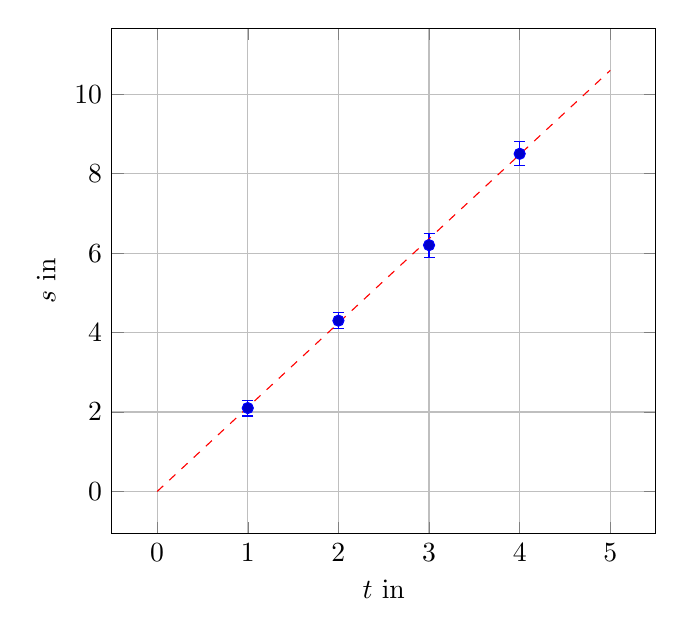
\begin{tikzpicture}
    \begin{axis}[
      width=0.7\textwidth,
      height=8cm,
      xlabel={$t$ in \si{\second}},
      ylabel={$s$ in \si{\milli\meter}},
      grid=major,
    ]
      \addplot+[
        only marks,
        error bars/.cd,
          x dir=both, x explicit,
          y dir=both, y explicit,
      ] coordinates {
        (1.0, 2.1) +- (0.0, 0.2)
        (2.0, 4.3) +- (0.0, 0.2)
        (3.0, 6.2) +- (0.0, 0.3)
        (4.0, 8.5) +- (0.0, 0.3)
      };
      \addplot+[domain=0:5, dashed, no marks] {2.12*x};
    \end{axis}
  \end{tikzpicture}
  \caption{Messwerte mit statistischen Unsicherheiten als Fehlerbalken
           sowie lineare Ausgleichsgerade $s = v \cdot t$ mit
           $v = (2{,}1 \pm 0{,}1)\,\si{\milli\meter\per\second}$.}
  \label{fig:fit}
\end{figure}
